%\documentclass{fhnwreport} %
%\usepackage[ngerman]{babel}
%\usepackage[T1]{fontenc}
%\usepackage[latin1]{inputenc}
%\usepackage{tikz}
%\usepackage{amsmath}
%\usetikzlibrary{arrows}
%\usepackage{lmodern}   %Type1-Schriftart f�r nicht-englische Texte 
%
%\usepackage{listings}
%\lstset{language=Matlab}
%
%\usepackage{color}
%
%% Farben f�r Matlab-Listings
%\definecolor{hellgelb}{rgb}{1,1,0.85}     % Hintergrundfarbe
%\definecolor{colKeys}{RGB}{0,0,255}       % blau
%\definecolor{colIdentifier}{RGB}{0,0,0}	  % schwarz
%\definecolor{colComments}{RGB}{34,139,34} % gruen
%\definecolor{colString}{RGB}{160,32,240}  % violett
%
%\lstset{%
    %language=Matlab,%
    %%backgroundcolor={\color{hellgelb}},%
		%backgroundcolor={},%
    %basicstyle={\footnotesize\ttfamily},%
    %breakautoindent=true,%
    %breakindent=10pt,%
    %breaklines=true,%
    %captionpos=t,%
    %columns=fixed,%
    %%commentstyle={\itshape\color{colComments}},%
		%commentstyle={\color{colComments}},
    %extendedchars=true,%
    %float=hbp,%
    %frame=single,%
    %framerule=1pt,%
    %identifierstyle={\color{colIdentifier}},%
    %keywordstyle={\color{colKeys}},%
    %numbers=left,%
    %numbersep=1em,%
    %numberstyle={\tiny\ttfamily},%
    %showspaces=false,%
    %showstringspaces=false,%
    %stringstyle={\color{colString}},%
    %tabsize=4,%
    %xleftmargin=1em,%
    %xrightmargin=1em%
%} 
%\graphicspath{{./PrettyPictures/}}
%
%\begin{document}
\subsubsection{Numerisches Beispiel PID-Regler }\label{PIDExample}
Die Berechnung eines PID-Reglers verl�uft �hnlich wie die eines PI-Reglers. F�r das Beispiel werden die gleichen Eingabeparameter verwendet wie beim PI-Regler:

$Ks=0.5$\\
$Tu=2.5$\\
$Tg=18.3$\\
$\phi_{Strecke}$=-114.6\textdegree\\

Im Gegensatz zum PI-Regler sind alle Ausgabeparameter in der bodekonformen Darstellung. Eine genauere Erkl�rung dazu ist im Anhang, Sektor \ref{Bodekonf}, Seite \pageref{Bodekonf} zu finden.

Zun�chst werden nun die Zeitkonstanten sowie die Ordnung der Strecke  mithilfe der Sani Methode bestimmt. Bei unserer Strecke ergibt dies eine Strecke 3.Ordnung und die folgenden Zeitkonstanten:

$T1=1.0688s$\\
\\
$T2=3.3484s$\\
\\
$T3=10.4901s$\\
\\
Nun wird der Frequenzgang aus der �bertragungsfunktion der Strecke \eqref{eq:�bertragungsfunktionStrecke} berechnet und in einem Plot aufgezeichnet (siehe Abbildung \ref{fig:PIDStep1}). Danach wird nach dem -135\textdegree ~Punkt auf dem Phasengang gesucht. Dieser ist mit der horizontalen blau gestrichelten Linie eingezeichnet und ergibt folgende Frequenz: $0.2987s^{-1}$.

\begin{figure}[h]	
\centering		
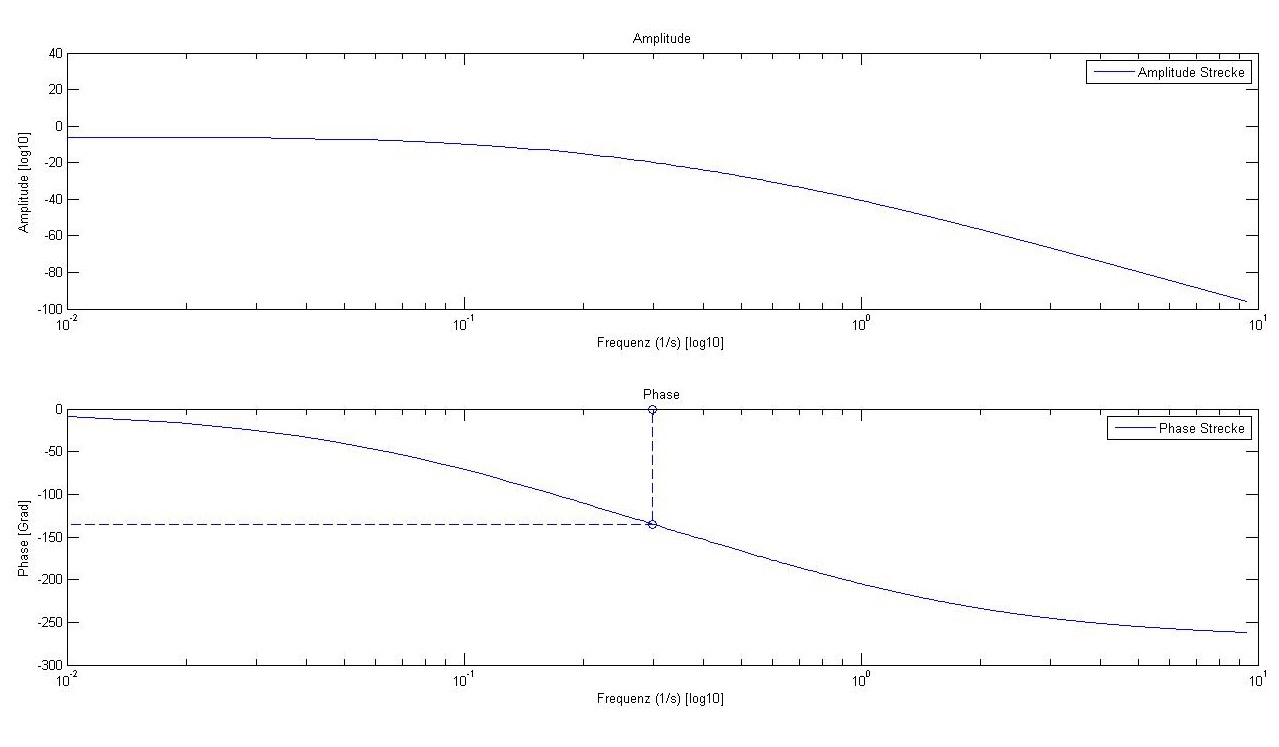
\includegraphics[width=1.0\textwidth]{PID_Step_01.jpg}
\caption{Amplituden- und Phasengang der Regelstrecke}	
\label{fig:PIDStep1}	
\end{figure}

\newpage
Bevor der Frequenzgang des offenen Regelkreises berechnet wird, muss $\beta$ bestimmt werden. Die Berechnung dazu ist im Anhang, Kapitel \ref{ZellwegerBeta} auf Seite \pageref{ZellwegerBeta} ersichtlich. Nach Ausf�hren dieser Berechnung erh�lt man $\beta=0.3192$.

Mit $\beta$ ist es m�glich, $Tnk=10.4902s$ und $Tvk=1.0688s$ zu berechnen.
Weiter wird noch $Tp$ bestimmt (siehe Kapitel \ref{ZellwegerMethode}, Seite \pageref{ZellwegerMethode}). In diesem Beispiel wurde $Tp$ eine Dekade kleiner als $Tvk$ gew�hlt, folglich ist der Wert von $Tp=0.107s$. 
Mit diesen Werten und $Krk =1$ wird nun der offene Amplituden- und Phasengang berechnet (Abbildung \ref{fig:PIDStep2}).

\begin{figure}[h]	
\centering		
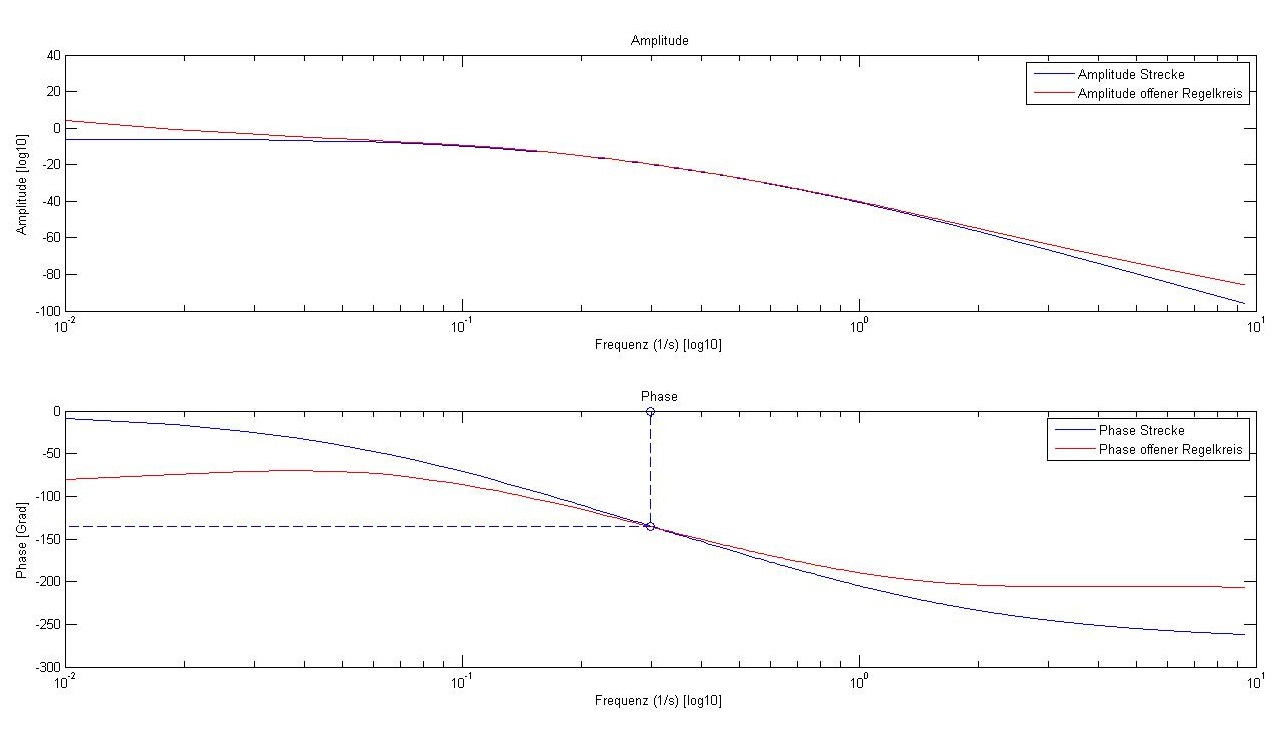
\includegraphics[width=1.0\textwidth]{PID_Step_02.jpg}
\caption{Frequenzgang der offenen Regelstrecke}	
\label{fig:PIDStep2}	
\end{figure}

%\newpage
Als n�chster Schritt wird die Tabelle \ref{table:Tab�berschwingen} auf Seite \pageref{table:Tab�berschwingen} zu Hilfe genommen. Daraus wird das gew�nschte �berschwingen ausgew�hlt und die entsprechende Frequenz auf dem Phasengang des offenen Regelkreises gesucht (siehe Abbildung \ref{fig:PIDStep3}). Die gefundene Frequenz betr�gt: $0.1317s^{-1}$.

\begin{figure}[h!]	
\centering		
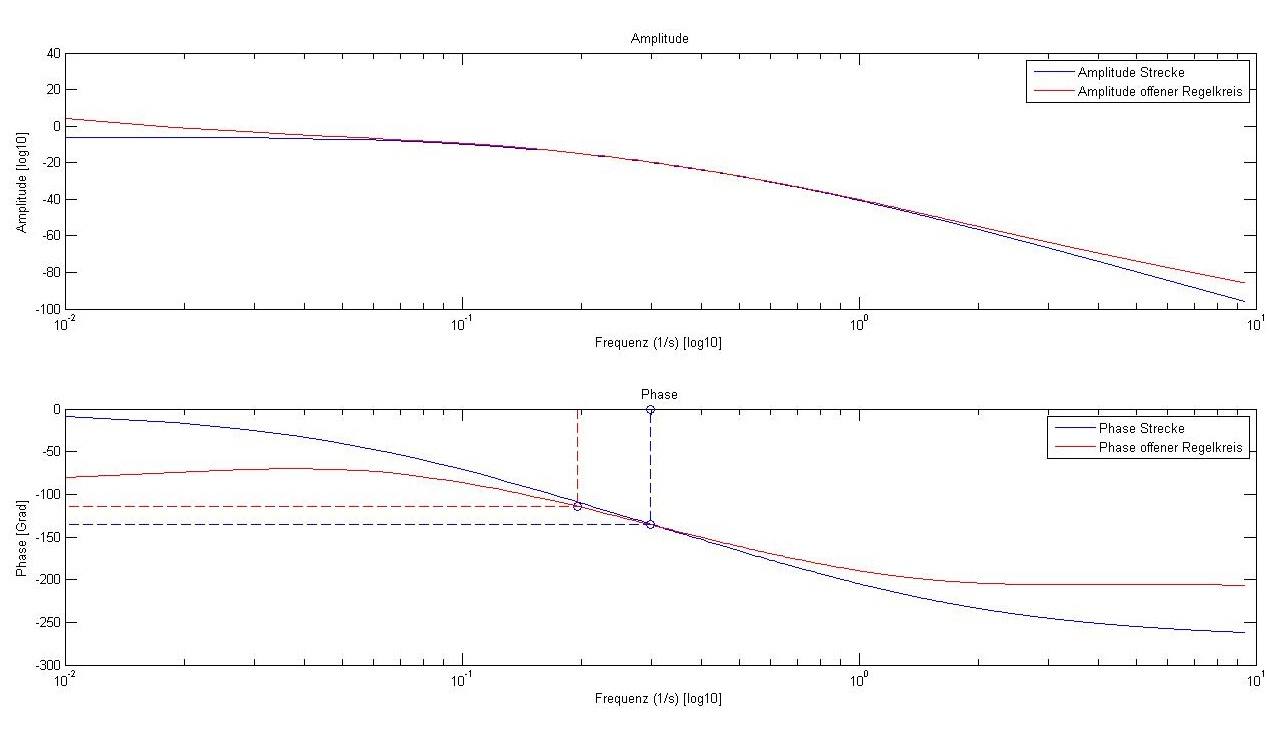
\includegraphics[width=1.0\textwidth]{PID_Step_03.jpg}
\caption{$\omega$ bei $\phi_{Strecke}$}	
\label{fig:PIDStep3}	
\end{figure}

\newpage
Zur gefundenen Frequenz liest man die Verst�rkung von $0.3312$ heraus. Der Kehrwert davon ergibt den letzten Faktor $Krk=3.0194$. (Abbildung \ref{fig:PIDStep4})

\begin{figure}[h!]	
\centering		
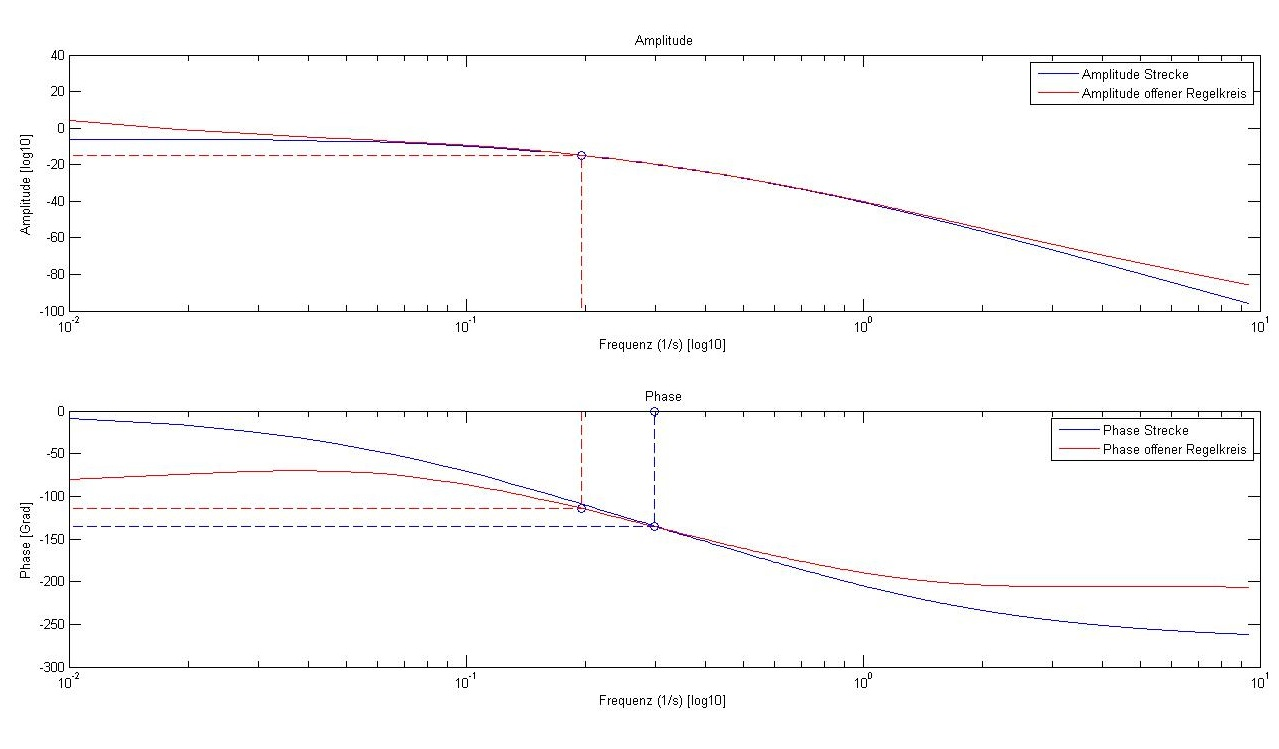
\includegraphics[width=1.0\textwidth]{PID_Step_04.jpg}
\caption{Bestimmung von $Krk$}	
\label{fig:PIDStep4}	
\end{figure}

\pagebreak
Die Endresultate dieser Berechnung sind:

$Tnk$ = 10.4902\\
$Tvk$ = 1.0688\\
$Krk$ = 3.0194

Wie schon erw�hnt, sind diese Angaben alle in der bodekonformen Darstellung. Umgewandelt in die reglerkonforme Darstellung ergibt dies folgende Werte:

$Tn =11.4521$\\
$Tv =0.8721$\\
$Kr =3.2963$

Den genauen Verlauf f�r die Umrechnung zur reglerkonformen Darstellung ist im Anhang, Sektor \ref{Bodekonf}, Seite \pageref{Bodekonf} zu finden.
	
%\end{document}